\section{Path constraints, boundary arcs, and hierarchical targets}
\label{sec:dynamic-constraints}

Time-optimal trajectories often contain interior arcs, converter-boundary
arcs, and switching points.  If only input magnitude is constrained and the
Hamiltonian is affine in voltage, the \gls{pmp} places the optimum on an
extreme point of \(\mathcal U\) almost everywhere.  In the smooth circular
case this means \(\|\vect u_s\|=U_{\max}\); with a hexagon it means a facet or
vertex.  The engineering statement ``unused voltage is unused local speed''
is therefore valid for pure minimum time on an unconstrained interior arc.  It
fails when a current, torque, thermal, slew, or terminal-manifold constraint
requires voltage headroom or creates a singular arc.

Relevant path constraints include
\begin{align}
 \|\vect i_s(t)\|&\leq I_{\max}, & |i_{\mathrm f}(t)|&\leq I_{\mathrm f,max},
 \tag{31.1}\\
 M(t)&\leq M_{\mathrm{target}}, & \dot M(t)&\geq0
 \quad\text{for a positive monotone step},
 \tag{31.2}
\end{align}
plus temperature and DC-link limits.  ``Only final torque matters'', ``no
overshoot'', ``monotonic torque'', and ``track torque throughout
reallocation'' define four different feasible path sets.  They must never be
reported as the same minimum-time problem.  The time-optimal MPC results of
\textcite{brosch2023} illustrate why current and torque constraints must be
included rather than repaired after an unconstrained time-optimal command.

\subsection{A two-stage EESM hypothesis}

Let \(A\) be the old loss-optimal point, \(B\) the new one, and \(C\) a rapidly
reachable point on the new torque surface.  The strategy
\[
 A\xrightarrow{\text{torque acquisition}}C
 \xrightarrow{\text{torque-neutral redistribution}}B
 \tag{31.3}
\]
is attractive when the stator subsystem is fast, the field subsystem slow,
the new torque surface can be reached with frozen field current, and enough
stator-current and voltage margin remains.  The second arc can use
\(\matr P_G\) to reduce loss without first-order torque error.  This resembles
the dynamic EESM current-allocation objective investigated by
\textcite{reinhard2024dynamic}.

It is exactly optimal only under restrictive separability: zero or compatible
drift, a target manifold reached by the fastest stator-only arc, no benefit
from simultaneous field motion, and a cost whose first priority is hitting
the torque surface.  With coupled inductance or field-voltage authority,
simultaneous motion can dominate.  The numerical experiment in
Section~\ref{sec:fast-slow-experiment} deliberately tests rather than assumes
the hypothesis.

\begin{figure}[tb]
\centering
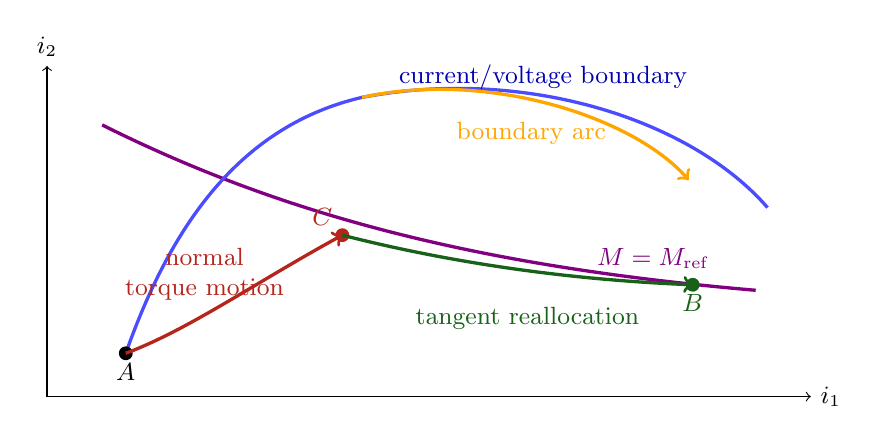
\begin{tikzpicture}[font=\small,x=1cm,y=1cm]
 \draw[->] (0,0)--(9.7,0) node[right] {$i_1$};
 \draw[->] (0,0)--(0,4.2) node[above] {$i_2$};
 \draw[Purple,very thick] (.7,3.45)..controls(3.0,2.3)and(5.5,1.65)..(9.0,1.35);
 \node[Purple] at (7.7,1.75) {$M=M_{\rm ref}$};
 \draw[blue!70,very thick] (1.0,.55)..controls(1.6,2.25)and(2.5,3.45)..(4.0,3.8)
   ..controls(6.1,4.2)and(8.2,3.5)..(9.15,2.4);
 \node[blue!70!black] at (6.3,4.05) {current/voltage boundary};
 \fill (1.0,.55) circle (2.5pt) node[below] {$A$};
 \fill[BrickRed] (3.75,2.05) circle (2.5pt) node[above left] {$C$};
 \fill[ForestGreen!70!black] (8.2,1.42) circle (2.5pt) node[below] {$B$};
 \draw[BrickRed,very thick,->] (1.0,.55)..controls(1.8,.85)and(2.65,1.45)..(3.75,2.05);
 \draw[ForestGreen!70!black,very thick,->] (3.75,2.05)..controls(5.2,1.68)and(6.7,1.48)..(8.2,1.42);
 \node[BrickRed,align=center] at (2.0,1.55) {normal\\torque motion};
 \node[ForestGreen!70!black] at (6.1,1.0) {tangent reallocation};
 \draw[Orange,very thick,->] (4.0,3.8)..controls(5.6,4.15)and(7.45,3.55)..(8.15,2.75);
 \node[Orange] at (6.15,3.35) {boundary arc};
\end{tikzpicture}
\caption{Two geometric structures that may coexist: hierarchical
torque acquisition followed by tangent reallocation, and a minimum-time
boundary arc that uses an active physical constraint as a road.}
\label{fig:two-stage-boundary}
\end{figure}



If torque has already been acquired, redistribution on \(\mathcal T\) may
ride a current or field-voltage boundary.  The induced tangent speed body is
the intersection of \(\mathcal V(\vect i)\) with the tangent plane
\(\nabla M^{\mathsf T}\dot{\vect i}=0\).  Its gauge supplies the exact local
travel-time density on the surface.  This construction handles both smooth
ellipsoids and converter polytopes without pretending that their geodesics
are identical.
